\documentclass[aspectratio=169,11pt]{beamer}
\usetheme{default}
\usecolortheme{seagull}
\setbeamertemplate{navigation symbols}{}
\setbeamertemplate{footline}[frame number]
\usepackage{booktabs,tikz}
\usetikzlibrary{positioning,arrows.meta}
\graphicspath{{../figures/}}

\title{Network Intrusion Detection on UNSW-NB15}
\subtitle{Integrated Project, Machine Learning (Prof.\ Youness Moukafih), Subject 13}
\author{Walid El Haimer \and Ayman Ezzougari \and Ahmed Ilyas Elmoussi \and Ahmed Graoui}
\institute{International University of Rabat}
\date{2026/2027}

\begin{document}

\begin{frame}
\titlepage
\end{frame}

%------------------------------------------------------------------
\begin{frame}{The task}
\begin{itemize}
\item Each sample is one network \textbf{flow}: 42 statistics (duration, bytes, packets, TTL, load,
counters, \texttt{proto}, \texttt{service}, \texttt{state}).
\item Official split: \textbf{175,341} training flows, \textbf{82,332} test flows.
\item Two questions:
  \begin{enumerate}
  \item Is the flow \textbf{normal or an attack}?
  \item If it is an attack, \textbf{which of 9 categories}? (incl.\ rare: Analysis, Backdoor,
  Shellcode, Worms)
  \end{enumerate}
\item Every alarm costs an analyst's time, so we fix an operating rule:\\[2pt]
\centering\fbox{\parbox{0.8\linewidth}{\centering at most \textbf{5\% of normal flows} may raise an alarm;\\
under that rule, catch as many attacks as possible}}
\end{itemize}
\end{frame}

%------------------------------------------------------------------
\begin{frame}{Our system: two stages}
\centering
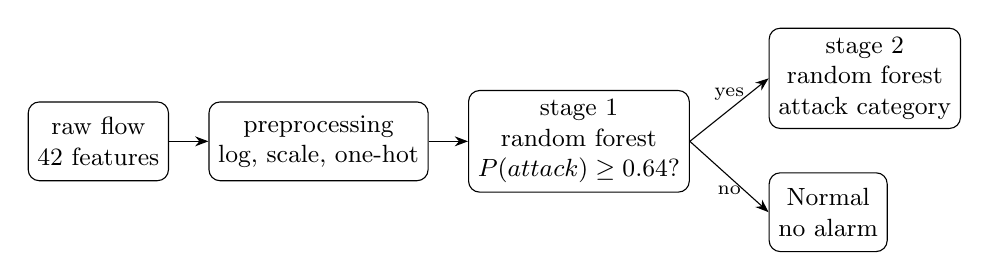
\begin{tikzpicture}[node distance=0.5cm, box/.style={draw, rounded corners, align=center,
  font=\small, minimum height=1cm}, >={Stealth}]
\node[box] (in) {raw flow\\42 features};
\node[box, right=of in] (prep) {preprocessing\\log, scale, one-hot};
\node[box, right=of prep] (bin) {stage 1\\random forest\\$P(\text{attack})\ge 0.64$?};
\node[box, right=1cm of bin, yshift=0.8cm] (cat) {stage 2\\random forest\\attack category};
\node[box, right=1cm of bin, yshift=-0.9cm] (norm) {Normal\\no alarm};
\draw[->] (in) -- (prep); \draw[->] (prep) -- (bin);
\draw[->] (bin.east) -- node[above, font=\scriptsize] {yes} (cat.west);
\draw[->] (bin.east) -- node[below, font=\scriptsize] {no} (norm.west);
\end{tikzpicture}
\vspace{0.5cm}
\begin{itemize}
\item Stage 1 carries the false alarm rule; stage 2 is trained on attack flows only.
\item The two answers can never contradict each other.
\end{itemize}
\end{frame}

%------------------------------------------------------------------
\begin{frame}{What the data looks like}
\begin{columns}
\column{0.52\textwidth}
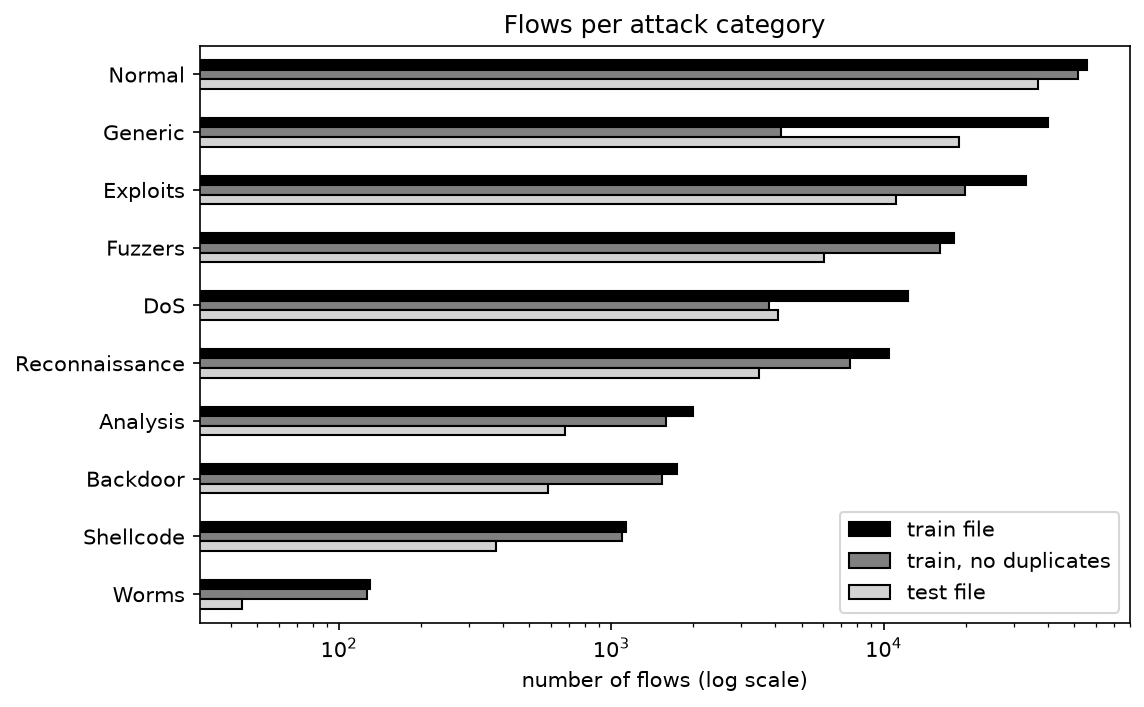
\includegraphics[width=\linewidth]{class_balance.png}
\column{0.46\textwidth}
\small
\begin{itemize}
\item No missing values.
\item \textbf{38.6\%} of training rows are exact duplicates (Generic: 40,000 $\to$ 4,181).
\item 1,772 identical flows carry 2+ categories: an error floor.
\item Strong imbalance: 51,890 normal vs.\ \textbf{127 Worms}.
\item Extremely skewed counts: \texttt{sbytes} median 430, max $1.3\times10^7$.
\item TTL 31 $\Rightarrow$ 0\% attacks, TTL 254 $\Rightarrow$ 90\% attacks.
\end{itemize}
\end{columns}
\end{frame}

%------------------------------------------------------------------
\begin{frame}{Preprocessing pipeline: each step has a reason}
\small
\begin{tabular}{p{0.38\linewidth}p{0.55\linewidth}}
\toprule
Step & Why \\
\midrule
Remove duplicates, then split 80/20 & copies on both sides of the split inflate validation \\
Stratified split by category & Worms (127 rows) must appear in train and validation \\
$\log(1+x)$ on numeric features & compresses counts spanning 7 orders of magnitude \\
Standardisation & features in seconds, bytes, flags: needed by distances and gradients \\
One-hot encoding (rare $\to$ ``infrequent'') & 133 protocols; state ACC/CLO only in the test file \\
Fitted inside a \texttt{Pipeline} on train only & no information leaks from validation or test \\
\bottomrule
\end{tabular}
\vspace{6pt}

\centering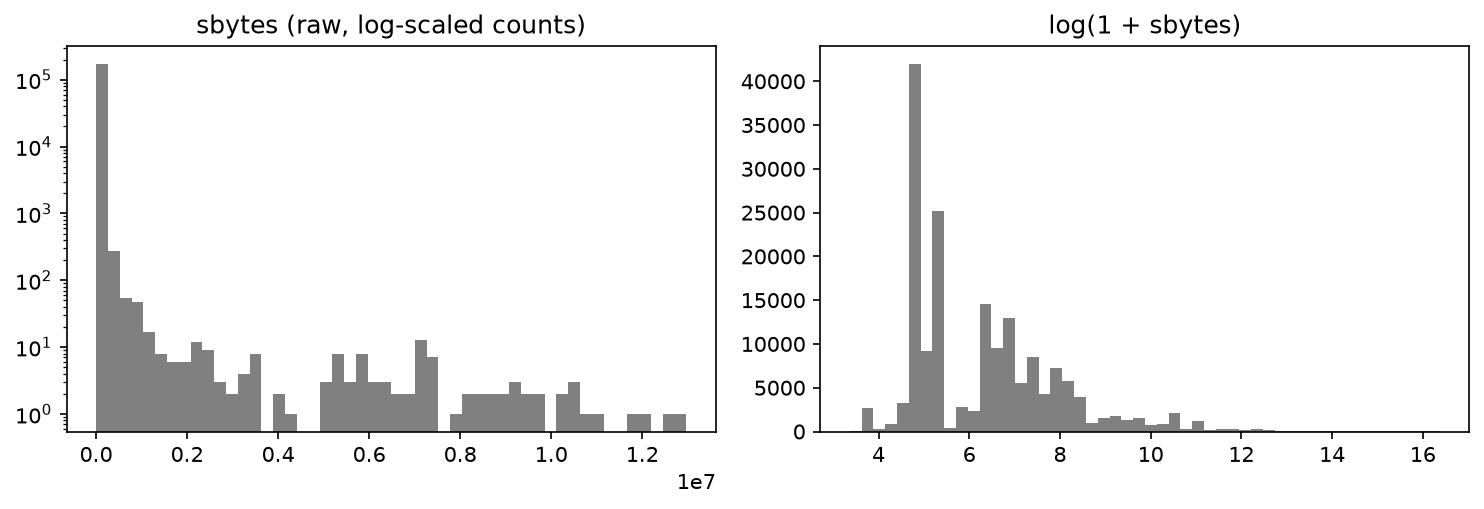
\includegraphics[width=0.5\linewidth]{log_transform.png}
\end{frame}

%------------------------------------------------------------------
\begin{frame}{Does it matter? A. Scaling (validation)}
\begin{columns}
\column{0.55\textwidth}
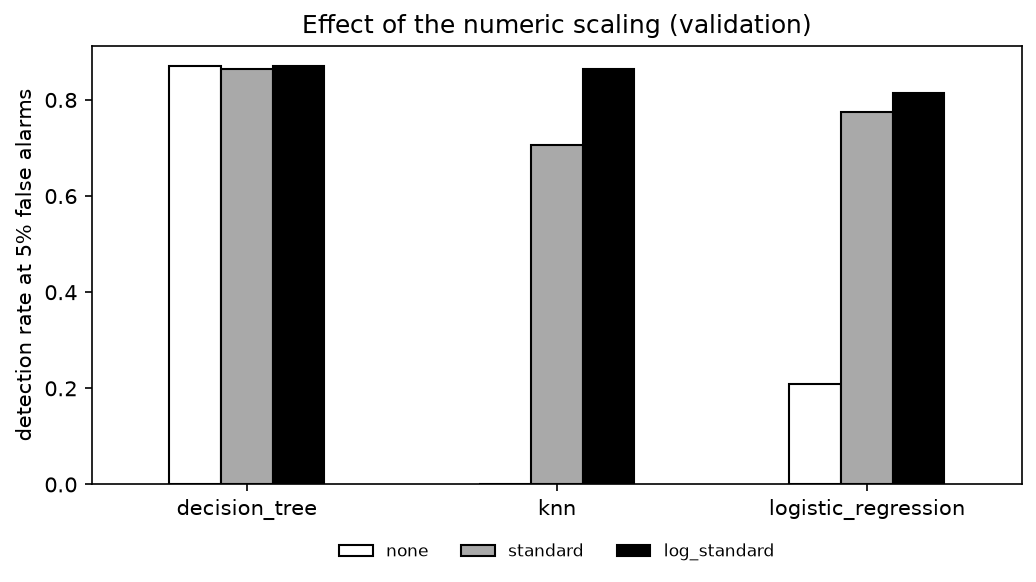
\includegraphics[width=\linewidth]{study_scaling.png}
\column{0.43\textwidth}
\small
Detection rate at 5\% false alarms:
\begin{itemize}
\item Logistic regression: 0.21 $\to$ 0.78 $\to$ \textbf{0.81}\\(unscaled: does not converge)
\item KNN: 0.00 $\to$ 0.71 $\to$ \textbf{0.87}\\(unscaled: cannot reach 5\%)
\item Decision tree: 0.87 in every case: a tree only compares a feature with a cut-off.
\end{itemize}
\end{columns}
\end{frame}

%------------------------------------------------------------------
\begin{frame}{Does it matter? B. Duplicates \quad C. TTL features}
\footnotesize
\begin{columns}[T]
\column{0.49\textwidth}
\textbf{B. Duplicates kept vs.\ removed}\\[3pt]
\begin{tabular}{lccc}
\toprule
 & Val det. & Test det. & Test FA \\
\midrule
LR removed & 0.814 & 0.906 & 0.136 \\
LR kept & \textbf{0.909} & 0.912 & 0.144 \\
RF removed & 0.908 & 0.964 & 0.168 \\
RF kept & \textbf{0.958} & 0.970 & 0.182 \\
\bottomrule
\end{tabular}\\[4pt]
Validation looks 5--10 points better, but the test score does not follow: the model was
recognising copies.
\column{0.49\textwidth}
\textbf{C. TTL features kept vs.\ dropped}\\[3pt]
\begin{tabular}{lccc}
\toprule
 & Val det. & Test det. & Test FA \\
\midrule
LR kept & 0.814 & 0.906 & 0.136 \\
LR dropped & 0.668 & 0.804 & 0.144 \\
RF kept & 0.908 & 0.964 & 0.168 \\
RF dropped & 0.902 & 0.958 & 0.162 \\
\bottomrule
\end{tabular}\\[4pt]
TTL is real signal for the linear model; dropping it does not fix the false alarms.
\end{columns}
\end{frame}

%------------------------------------------------------------------
\begin{frame}{Models and hyperparameter search}
\footnotesize
Course models; full grid; every candidate trained on train, scored on validation.\\[4pt]
\begin{tabular}{lll}
\toprule
 & Stage 1 search space & Stage 2 search space \\
\midrule
Logistic regression & $C\in\{0.01,0.1,1,10\}$ & $C\in\{0.1,1,10\}$, class weight \\
Decision tree & depth $\in\{5,10,20,\infty\}$, leaf $\in\{1,10\}$ & depth $\in\{10,20,\infty\}$, leaf, class weight \\
Random forest & depth $\in\{10,20\}$, leaf $\in\{1,5\}$ & depth 20, leaf $\in\{1,5\}$, class weight \\
\midrule
Score & detection rate at $\le$5\% false alarms & macro F1 (rare classes count) \\
\midrule
\textbf{Best} & \textbf{RF, depth 20: 0.908}, threshold 0.64 & \textbf{RF, balanced: 0.602} \\
\bottomrule
\end{tabular}\\[6pt]
\begin{itemize}
\item Threshold = lowest $t$ with $\le$5\% of normal validation flows above it.
\item A fully grown tree has pure leaves (probabilities 0 or 1): it can never meet the 5\% rule, so it is rejected.
\end{itemize}
\end{frame}

%------------------------------------------------------------------
\begin{frame}{Results, stage 1: detection on the test set}
\begin{columns}
\column{0.58\textwidth}
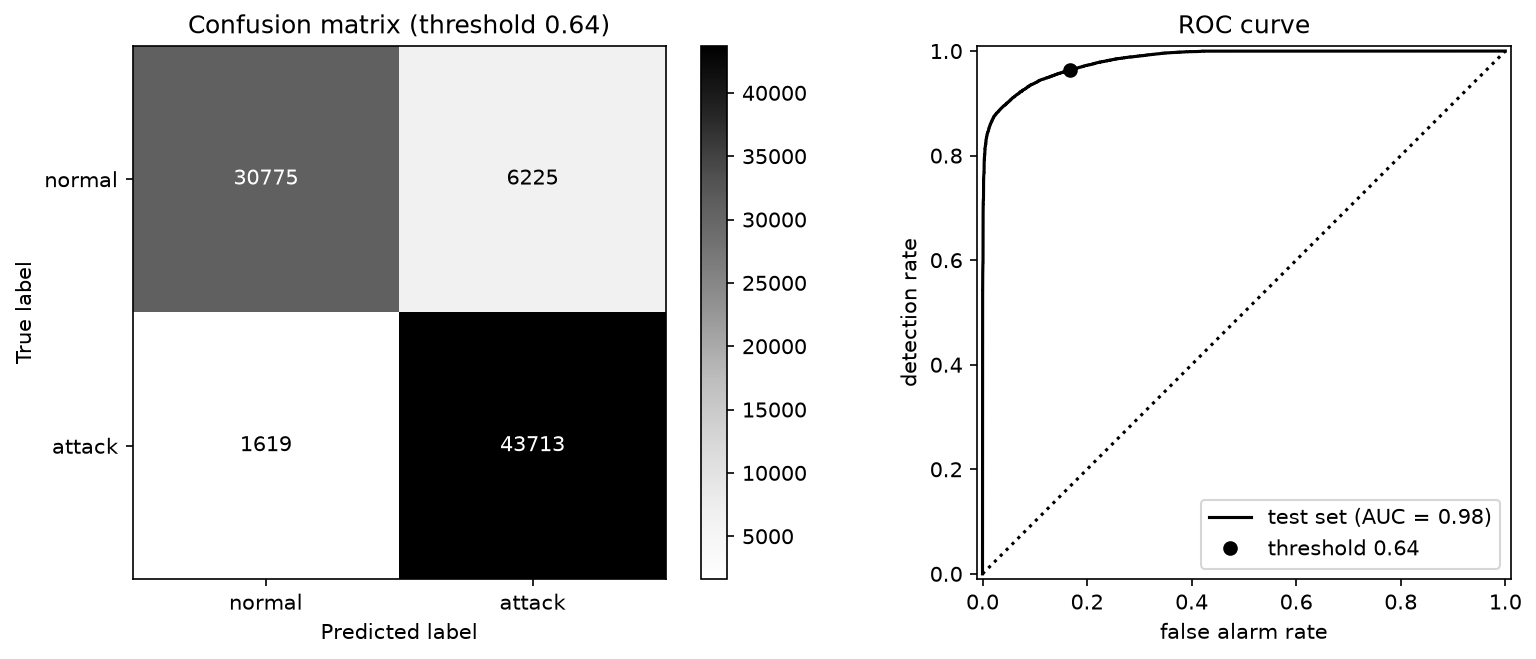
\includegraphics[width=\linewidth]{test_confusion_roc.png}
\column{0.4\textwidth}
\footnotesize
\begin{tabular}{lcc}
\toprule
threshold & 0.5 & \textbf{0.64} \\
\midrule
detection rate & 0.987 & 0.964 \\
precision & 0.816 & 0.875 \\
false alarm rate & 0.273 & \textbf{0.168} \\
F1 & 0.893 & 0.918 \\
ROC AUC & \multicolumn{2}{c}{0.983} \\
\bottomrule
\end{tabular}\\[4pt]
Every category is caught at 97--100\%, except \textbf{Fuzzers (75.8\%)}.
\end{columns}
\end{frame}

%------------------------------------------------------------------
\begin{frame}{Why 16.8\% false alarms instead of 5\%?}
\begin{columns}
\column{0.5\textwidth}
\small
Normal flows by source TTL:\\[3pt]
\begin{tabular}{lcccc}
\toprule
TTL & 0 & 31 & 62 & 254 \\
\midrule
train file & 5.1\% & 70.5\% & 3.9\% & 20.1\% \\
test file & 2.7\% & 45.1\% & 11.2\% & \textbf{40.7\%} \\
false alarms & 0\% & 0\% & 11.8\% & \textbf{38.1\%} \\
\bottomrule
\end{tabular}
\column{0.48\textwidth}
\small
\begin{itemize}
\item In training, TTL 254 means attack 90\% of the time.
\item The test file has twice as many normal TTL-254 flows.
\item $\Rightarrow$ \textbf{distribution shift}: validation (same file as training) could not see it.
\item Fix in practice: re-calibrate the threshold on recent normal traffic.
\end{itemize}
\end{columns}
\end{frame}

%------------------------------------------------------------------
\begin{frame}{Results, stage 2: attack categories and rare classes}
\begin{columns}
\column{0.45\textwidth}
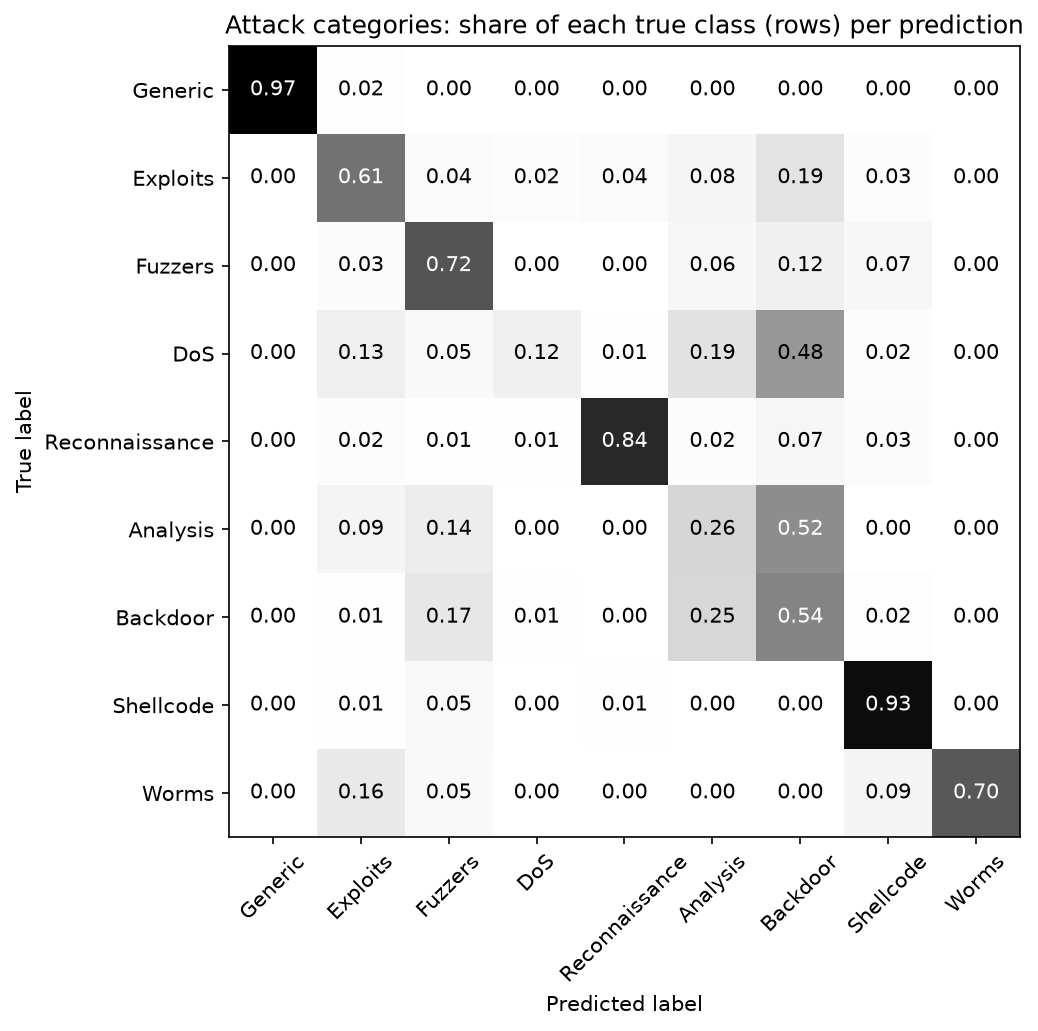
\includegraphics[width=\linewidth]{test_multiclass_confusion.png}
\column{0.53\textwidth}
\footnotesize
\begin{tabular}{lccc}
\toprule
test attacks & recall & precision & F1 \\
\midrule
Generic & 0.971 & 0.998 & 0.984 \\
Reconnaissance & 0.839 & 0.869 & 0.853 \\
Shellcode (378) & 0.926 & 0.269 & 0.417 \\
Worms (44) & 0.705 & 0.517 & 0.596 \\
DoS & \textbf{0.120} & 0.570 & 0.198 \\
Analysis & 0.257 & 0.072 & 0.112 \\
Backdoor & 0.544 & 0.056 & 0.101 \\
\midrule
macro avg & 0.632 & 0.558 & 0.526 \\
\bottomrule
\end{tabular}\\[4pt]
DoS, Analysis, Backdoor and Exploits share the same flow statistics, so they cannot be
separated from these features.
\end{columns}
\end{frame}

%------------------------------------------------------------------
\begin{frame}{Limitations and future work}
\begin{itemize}
\item \textbf{Distribution shift}: 5\% false alarms on validation $\to$ 16.8\% on test.
Re-calibrate on recent traffic; monitor the false alarm rate.
\item \textbf{Ambiguous categories}: merge DoS/Analysis/Backdoor/Exploits, or add packet-level
features, or show the top-2 categories to the analyst.
\item \textbf{Rare classes}: compare oversampling with class weights.
\item \textbf{Evaluation}: $k$-fold cross-validation for error bars; wider search grid.
\item \textbf{Models}: gradient boosting / AdaBoost from the course.
\end{itemize}
\vspace{6pt}
\centering\fbox{\parbox{0.8\linewidth}{\centering Main lesson: careful preprocessing (duplicates,
log scaling) and an honest look at false alarms matter more than the choice of model.}}
\end{frame}

\begin{frame}
\centering\Large Thank you\\[8pt]
\normalsize Code: \texttt{python main.py} (train) \quad \texttt{python test.py} (test / inference)
\end{frame}

\end{document}
